\documentclass[14pt, fleqn, xcolor={dvipsnames, table}]{beamer}
\usepackage[T2A]{fontenc}
\usepackage[utf8]{inputenc}
\usepackage[english,russian]{babel}
\usepackage{amssymb,amsfonts,amsmath,mathtext}
\usepackage{cite,enumerate,float,indentfirst}
\usepackage{cancel}
\usepackage{color}
\usepackage{hyperref}
\hypersetup{colorlinks,urlcolor=NavyBlue}

\usepackage{tikz}                   
\usetikzlibrary{shadows}

% \usepackage{enumitem}
% \setitemize{label=\usebeamerfont*{itemize item}%
%   \usebeamercolor[fg]{itemize item}
%   \usebeamertemplate{itemize item}}

\graphicspath{{images/}}

\usetheme{Boadilla}
\usecolortheme{seahorse}
\usefonttheme{serif}
\renewcommand{\CancelColor}{\color{red}}

\setbeamercolor{footline}{fg=Blue!50}
\setbeamertemplate{footline}{
  \leavevmode%
  \hbox{%
  \begin{beamercolorbox}[wd=.333333\paperwidth,ht=2.25ex,dp=1ex,center]{}%
    Амосов Федор, СПбГУ
  \end{beamercolorbox}%
  \begin{beamercolorbox}[wd=.333333\paperwidth,ht=2.25ex,dp=1ex,center]{}%
    Санкт-Петербург, 2014
  \end{beamercolorbox}%
  \begin{beamercolorbox}[wd=.333333\paperwidth,ht=2.25ex,dp=1ex,right]{}%
  Стр. \insertframenumber{} из \inserttotalframenumber \hspace*{2ex}
  \end{beamercolorbox}}%
  \vskip0pt%
}
\newcommand\indentdisplays[1]{%
     \everydisplay{\addtolength\displayindent{#1}%
     \addtolength\displaywidth{-#1}}}
\newcommand{\itemi}{\item[\checkmark]}

\title{Определение параметров межзвездного поглощения света по данным каталога Hipparcos\\\small{}}
\author[]{
    \small{
        Амосов Федор, СПбГУ\\
    }
}
\date{}

\begin{document}

    \begin{frame}
        \maketitle
        \small
    \end{frame}
    
     \section{Постановка задачи} 

        \begin{frame}{Постановка задачи}
            Дан звездный каталог с данными о
            \begin{itemize}
                \item положениях
                \item параллаксах
                \item фотометрии
                \item спектральных классах и классах светимости
            \end{itemize}  
            Задача
            \begin{itemize}
                \item Построить трехмерную карту пылевых облаков 
            \end{itemize}         
        \end{frame}
        
        \begin{frame}{Каталог}
            Звездный каталог с данными о
            \begin{itemize}
                \item положениях
                \item параллаксах
                \item фотометрии
                \item спектральных классах и классах светимости
            \end{itemize}  
            $\Longrightarrow$ каталог Hipparcos ($10^5$ звезд)
        \end{frame}
        
        \begin{frame}{Покраснение}
            $$
                E_{B - V} = (B - V)_{obs} - (B - V)_{int}
            $$
            Пример на звезде HIP 44800
            \begin{itemize}
                \item У нее в каталоге $(B - V)_{obs} = 0.535^m$
                \item Класс F7V, поэтому$^*$ $(B - V)_{int} = 0.493^m$
                \item Покраснение $0.535^m - 0.493^m = 0.042^m$
                \item Между нами и звездой пыли на $0.042^m$
            \end{itemize}
        \end{frame}    

    \section{Зависимость покраснения от расстояния}     
    
        \begin{frame}{Идеальная кривая покраснения}
            \begin{center}
                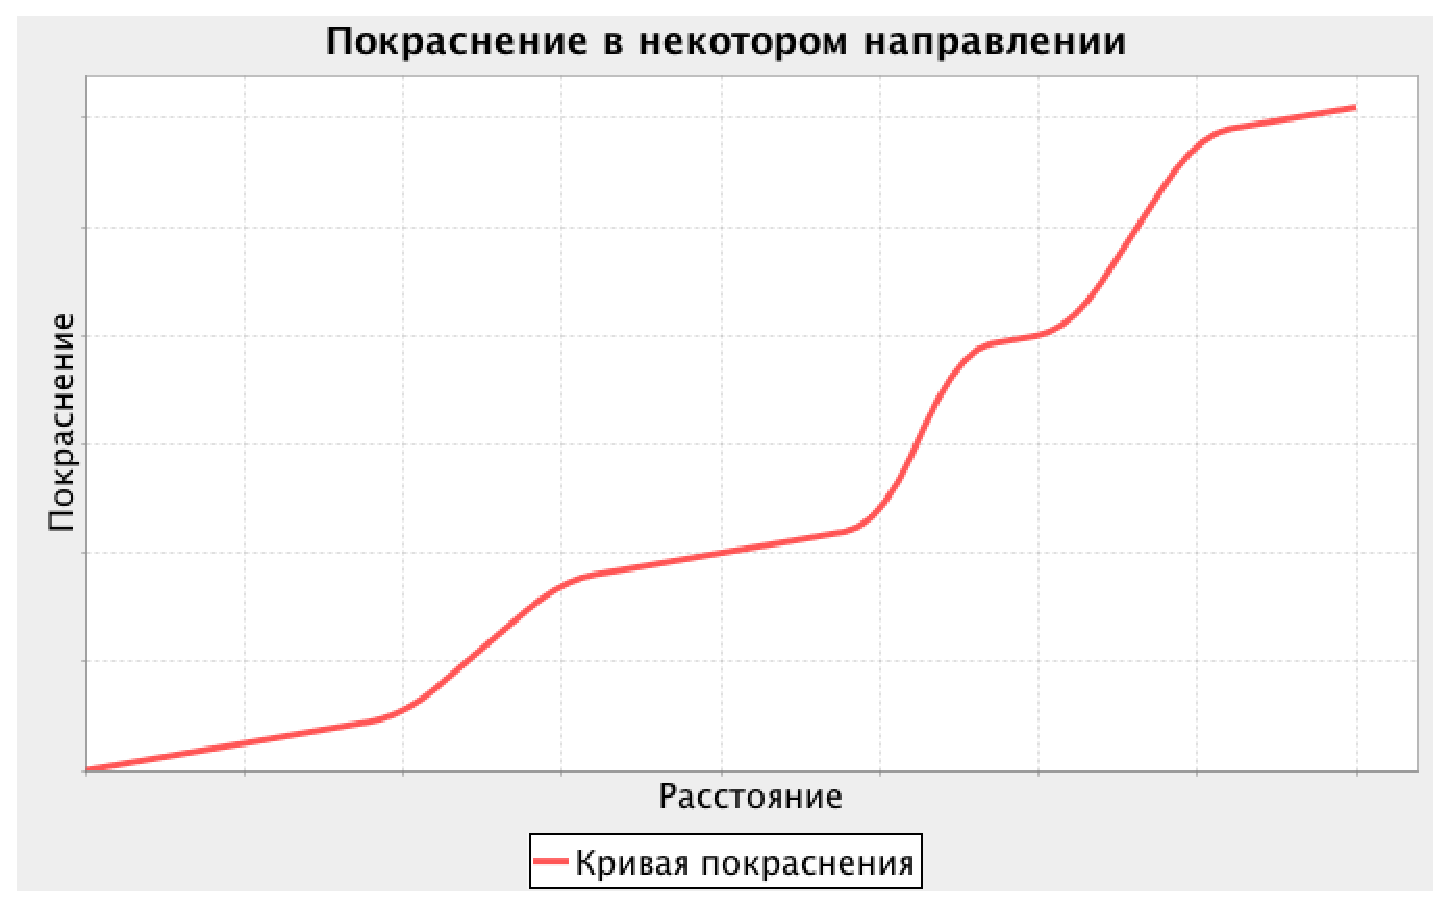
\includegraphics[width=11cm]{ideal-1-no-tick.eps}
            \end{center}             
        \end{frame}
        
        \begin{frame}{Пылевые облака}
            \begin{center}
                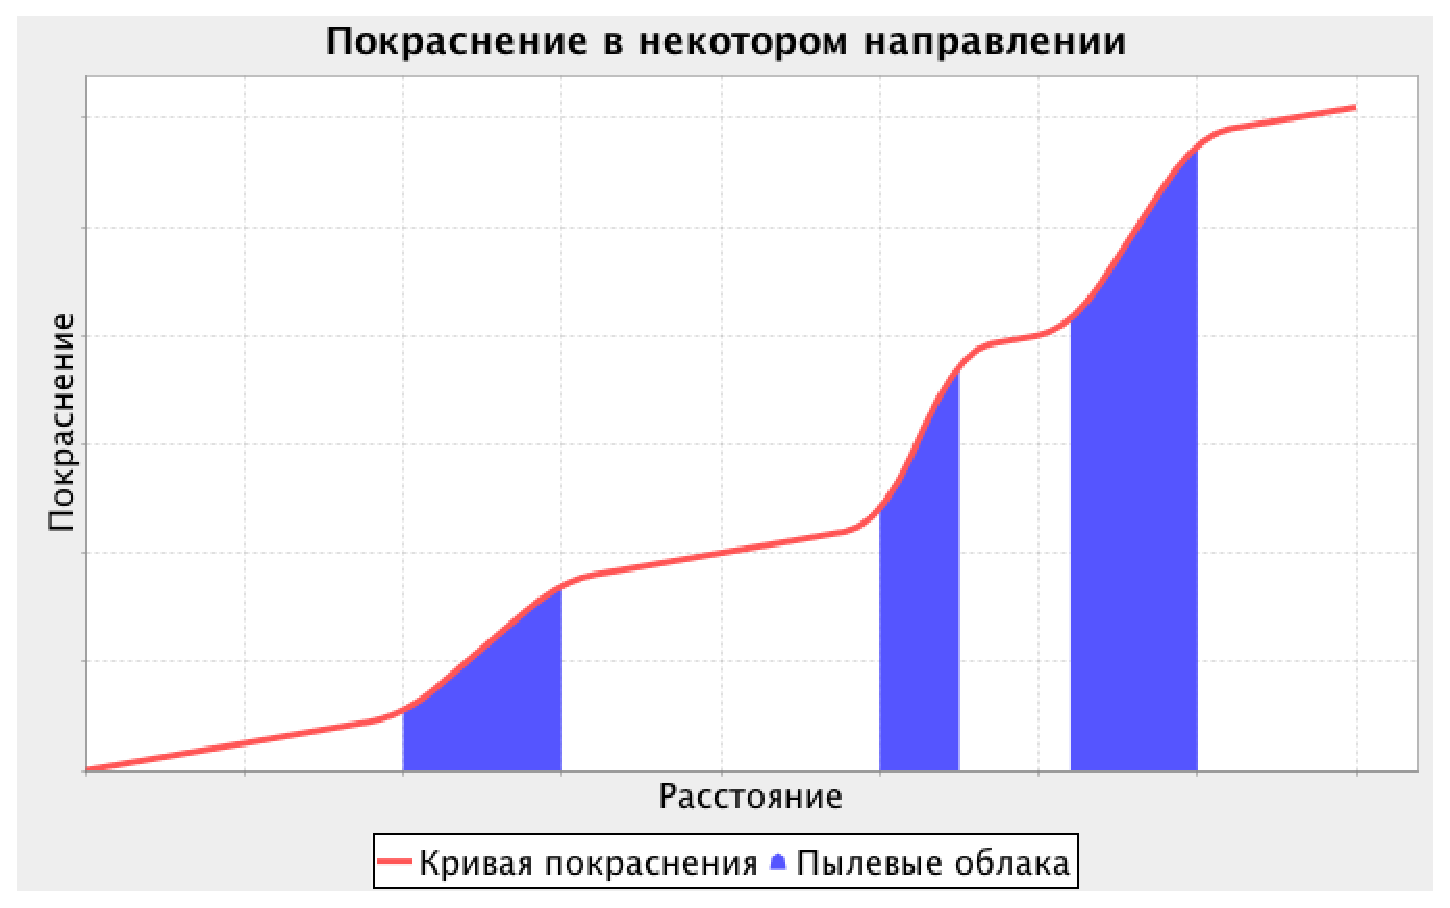
\includegraphics[width=11cm]{ideal-2-no-tick.eps}
            \end{center}             
        \end{frame}
        
        \begin{frame}{Реальное покраснение}
            \begin{center}
                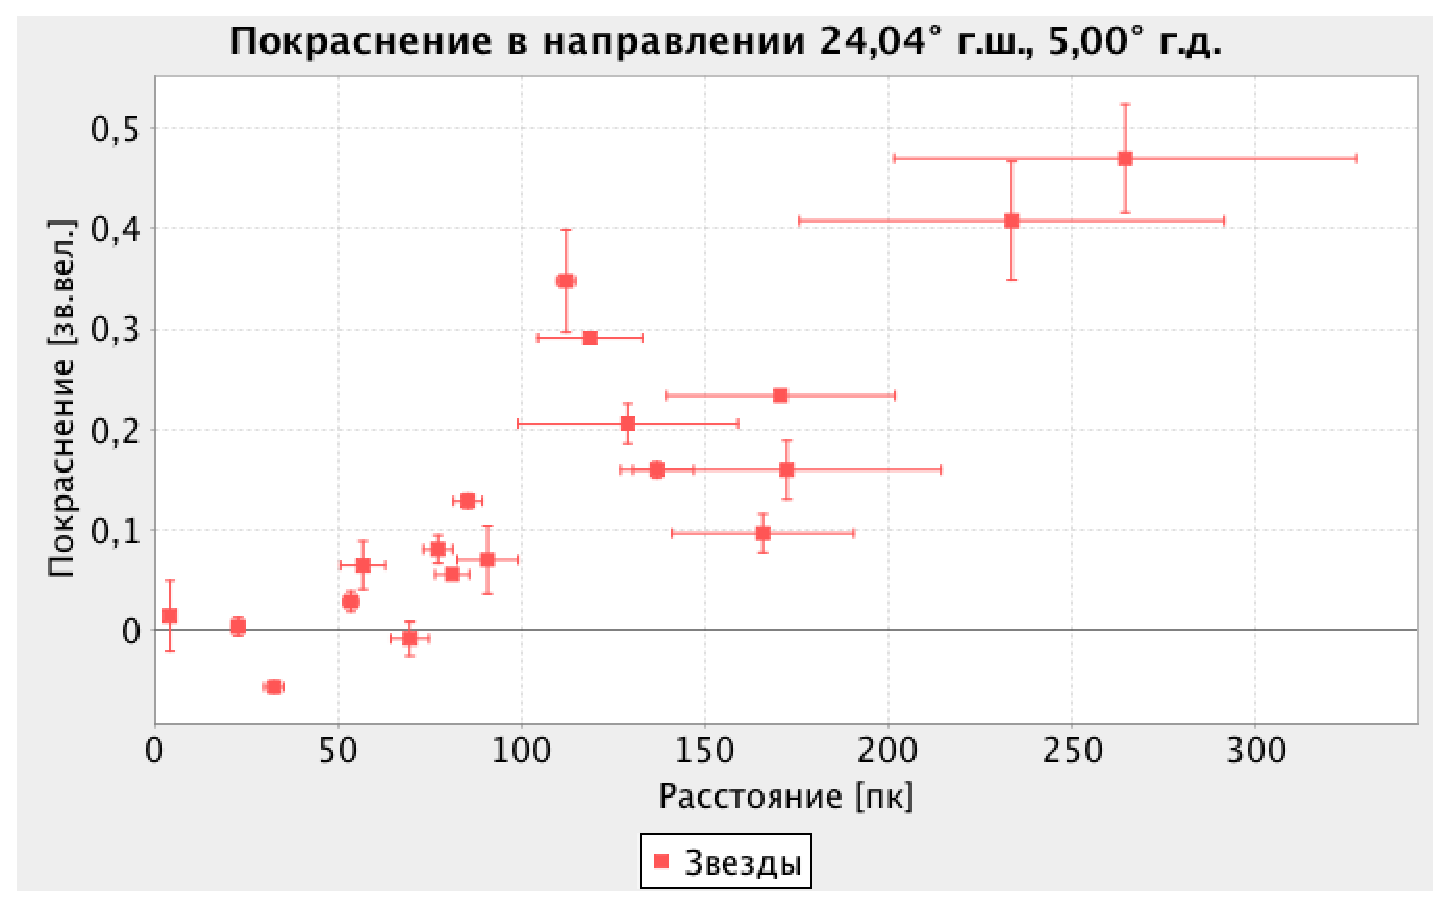
\includegraphics[width=11cm]{real-1.eps}
            \end{center}             
        \end{frame}
        
        \begin{frame}{Реальная <<кривая>> покраснения}
            \begin{center}
                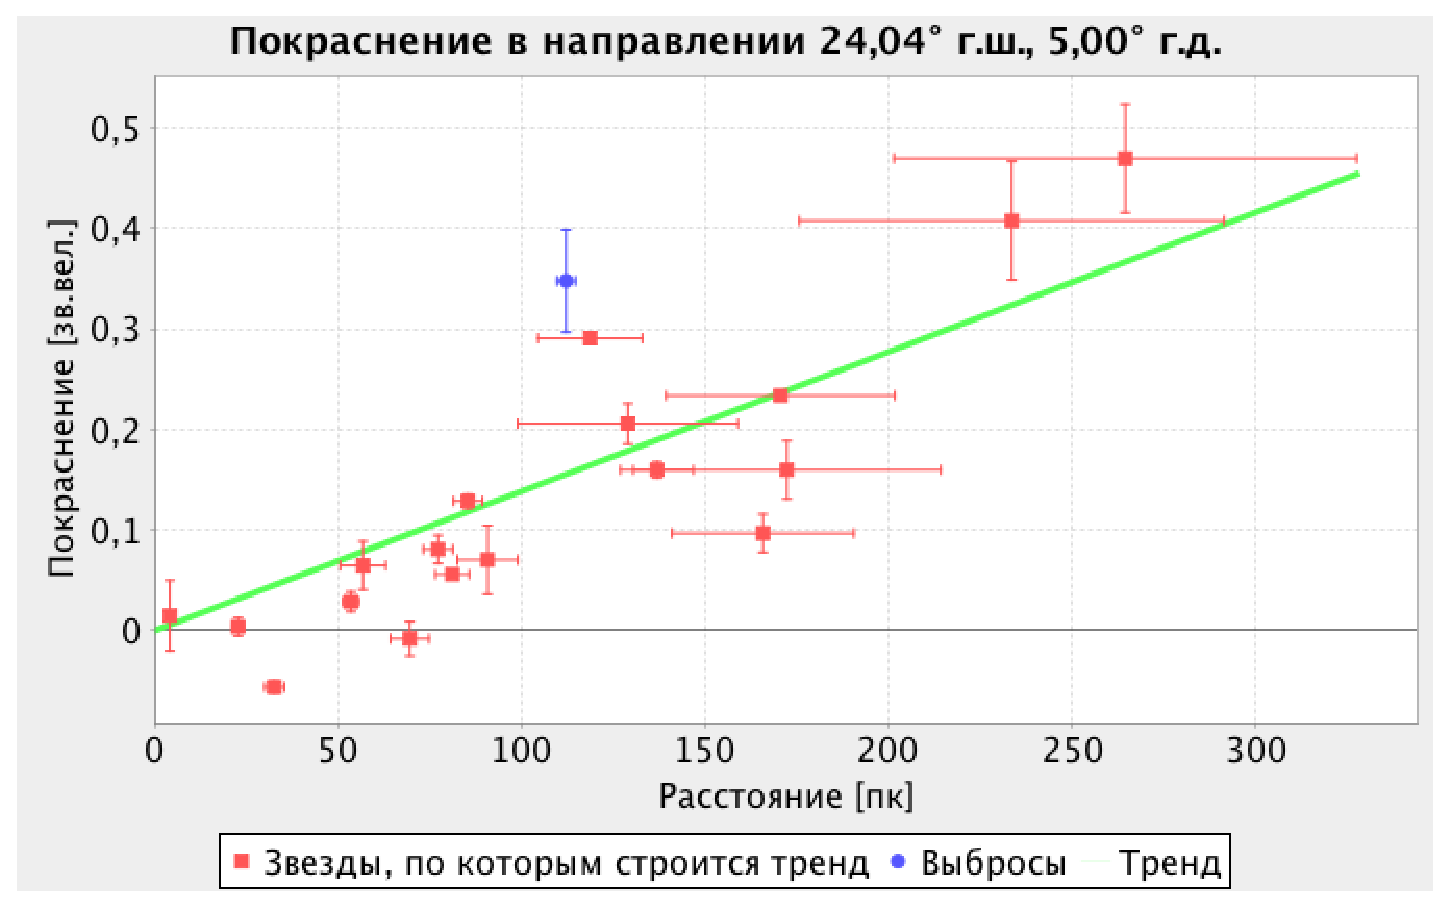
\includegraphics[width=11cm]{real-2-k.eps}
            \end{center}             
        \end{frame}
        
        \begin{frame}{<<В среднем>>}
            \begin{center}
                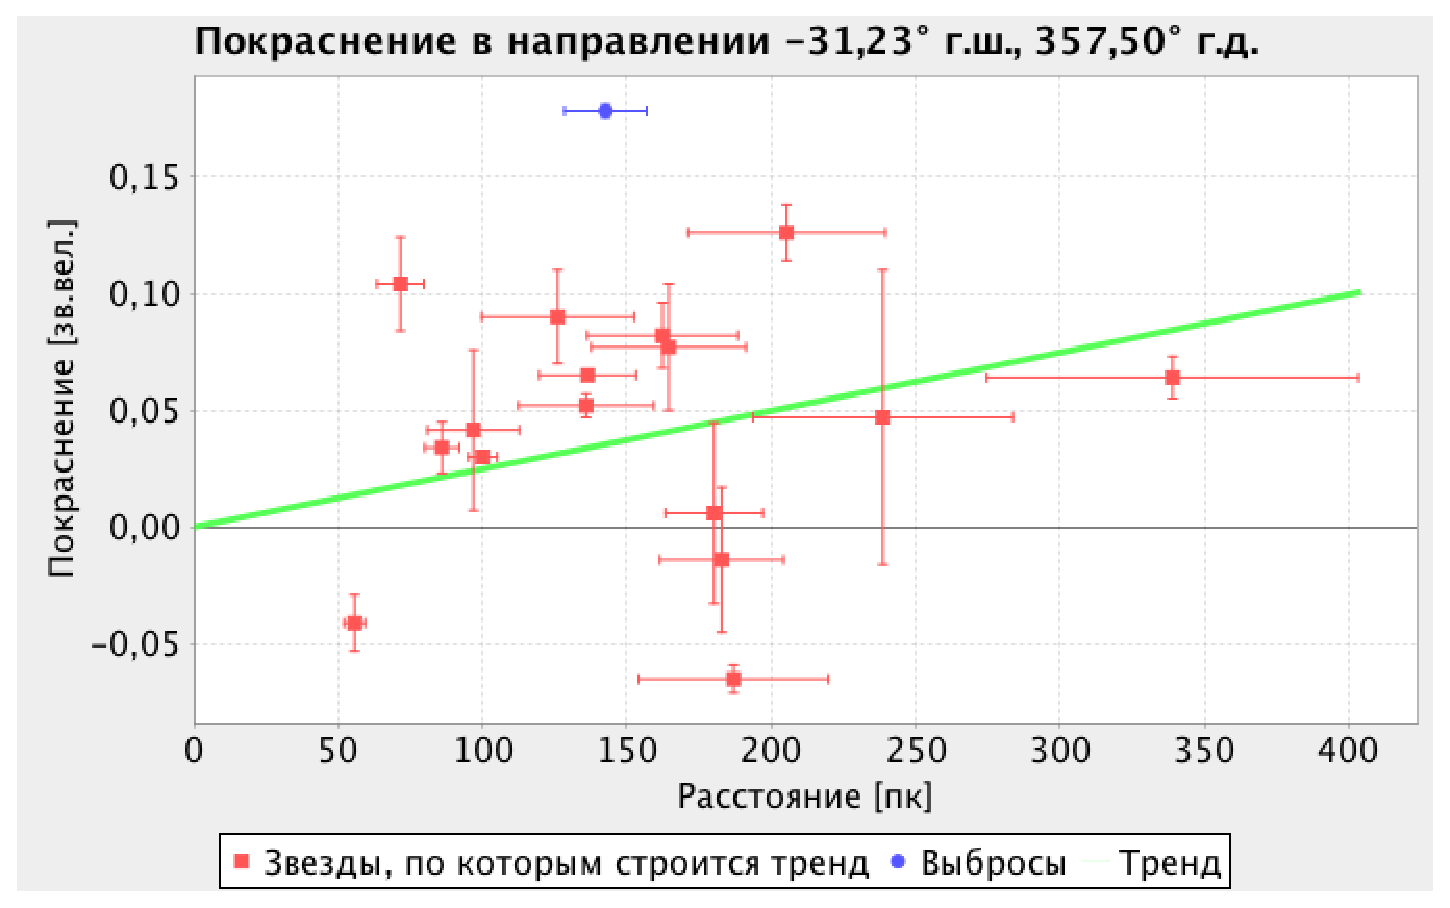
\includegraphics[width=11cm]{real-3-k.eps}
            \end{center}             
        \end{frame}        
        
        \begin{frame}{Отрицательный тренд}
            \begin{center}
                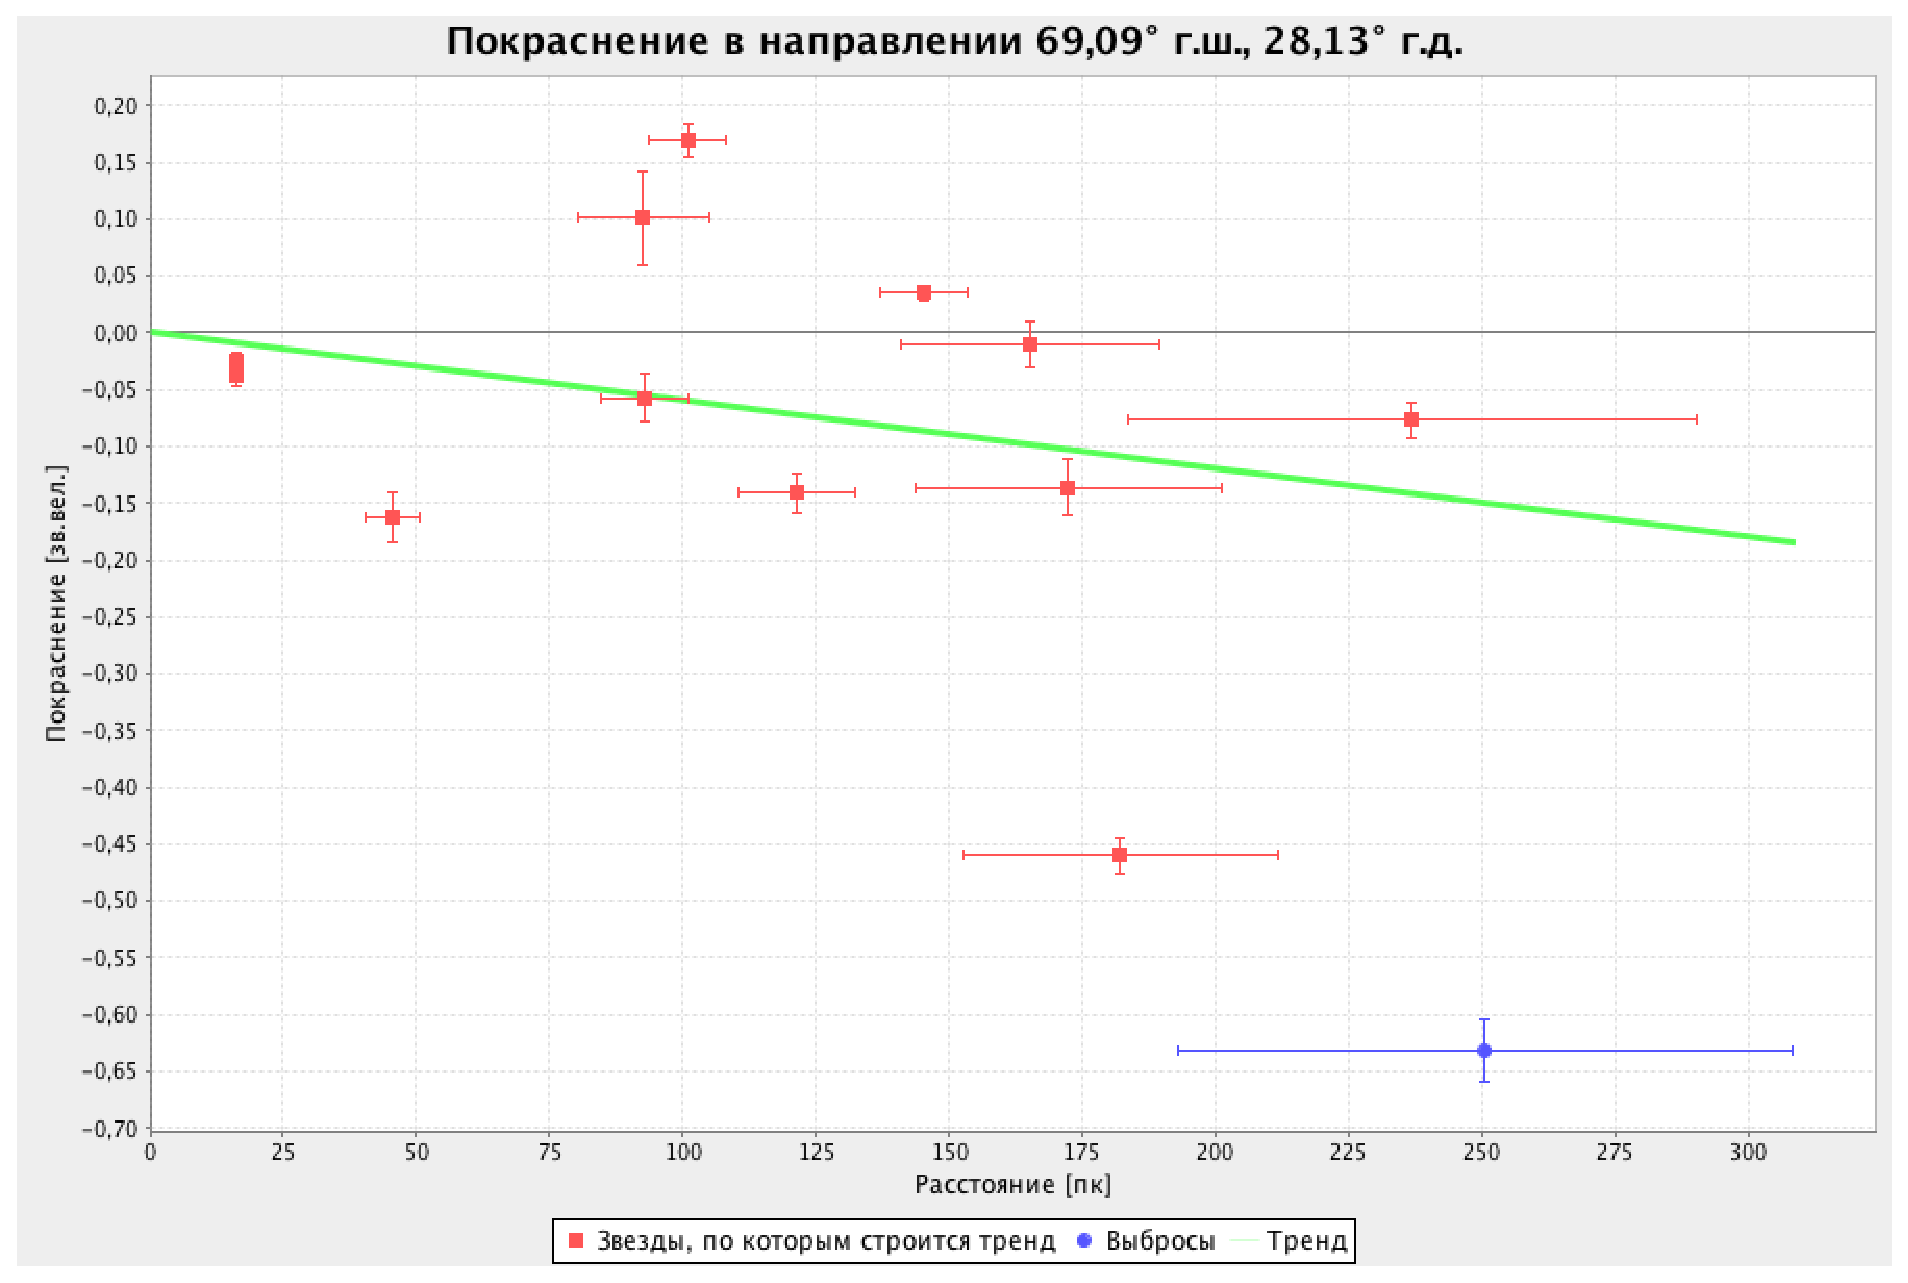
\includegraphics[width=11cm]{real-4-k.eps}
            \end{center}             
        \end{frame}
        
    \section{Карты}            
        
        \begin{frame}{Коэффициент $k$ ~~~~~~~~~~~~~~~~ $E_{B - V} = k r$}
            \begin{center}
                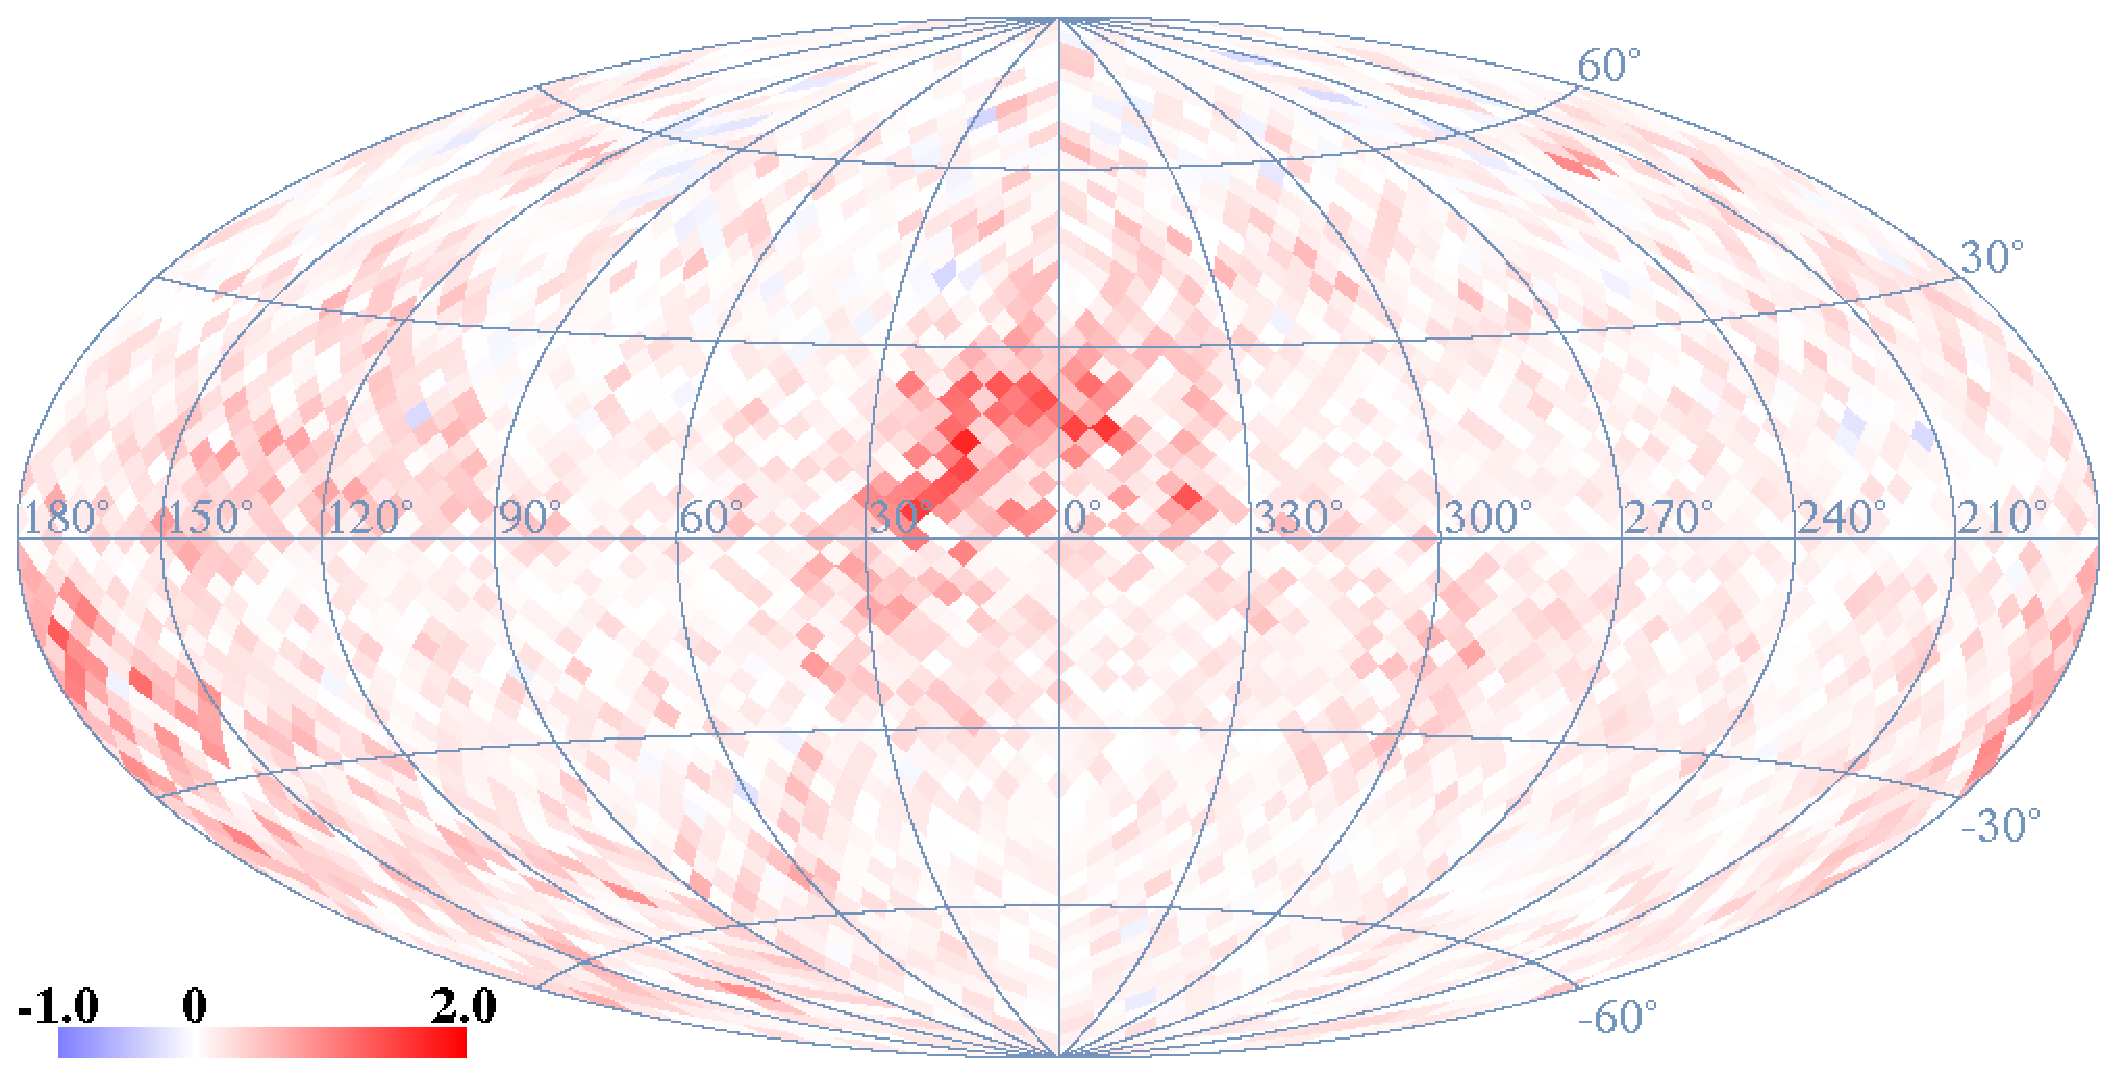
\includegraphics[width=11cm]{map-k.eps}
            \end{center}             
        \end{frame}
        
        \begin{frame}{$k / \sigma_k > 2$}
            \begin{center}
                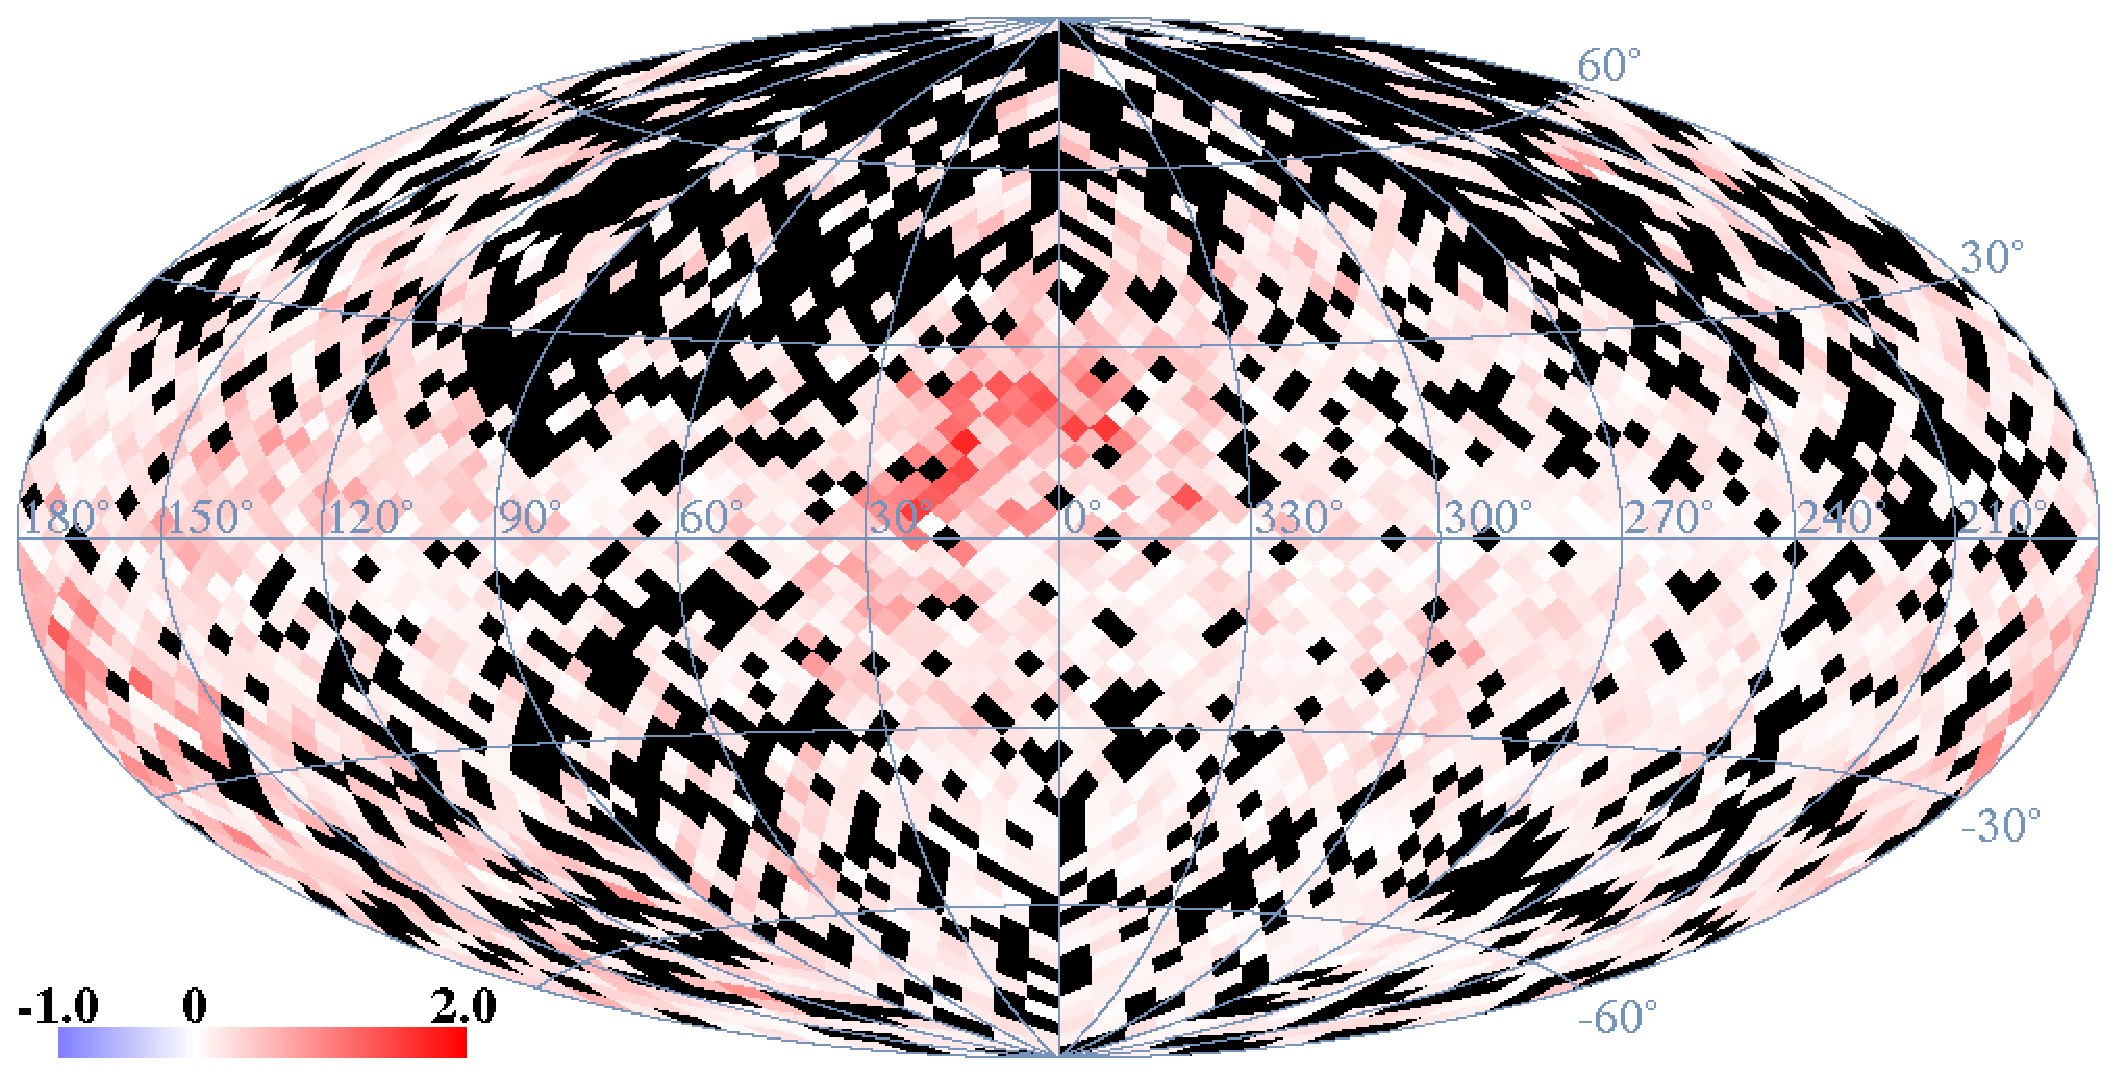
\includegraphics[width=11cm]{map-k-2sigma.eps}
            \end{center}             
        \end{frame}
        

    \section{Предварительная обработка}                
        
        \begin{frame}{Предварительная обработка}
            \begin{itemize}
                \item В расчет берутся $94199$ из $118219$ звезд
                \item Разбиение сферы на $12 \cdot 18^2 = 3888$ равновеликих частей алгоритмом Healpix
                \item Тренды строятся по 90\% расчетных звезд
                \item Расчет отсутствующих классов светимости
                \begin{itemize}
                    \item Спектральный класс, класс светимости $\Longrightarrow (B - V)_{int}$
                \end{itemize}
            \end{itemize}
        \end{frame}
        
        \begin{frame}{Наличие классов светимости}
            \begin{center}
                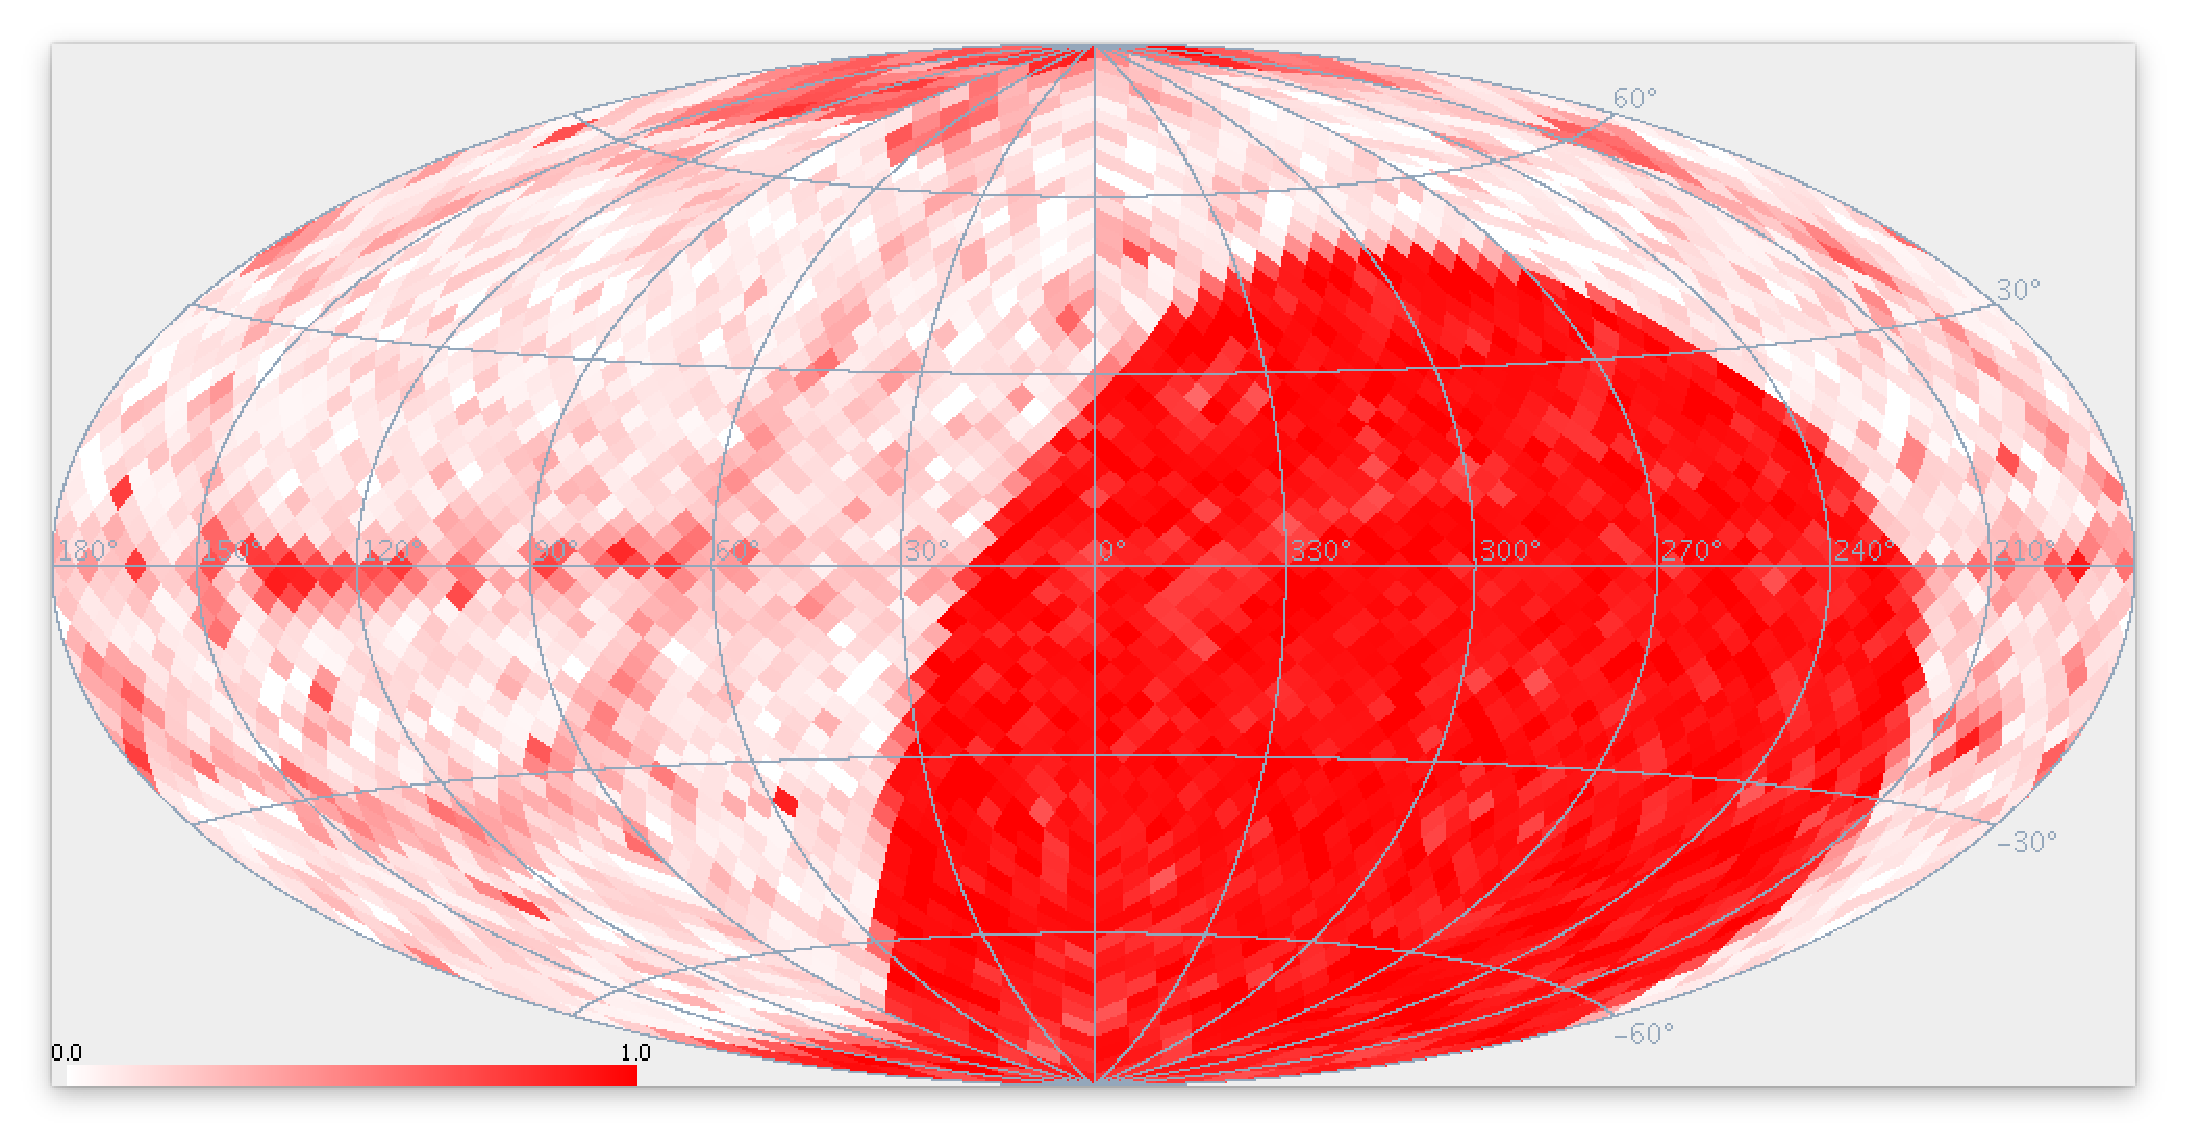
\includegraphics[width=11cm]{has-lumin.eps}
            \end{center}             
        \end{frame}

    \section{Определение классов светимости}                
        
        \begin{frame}{Обучение классификатора}
            \begin{center}
                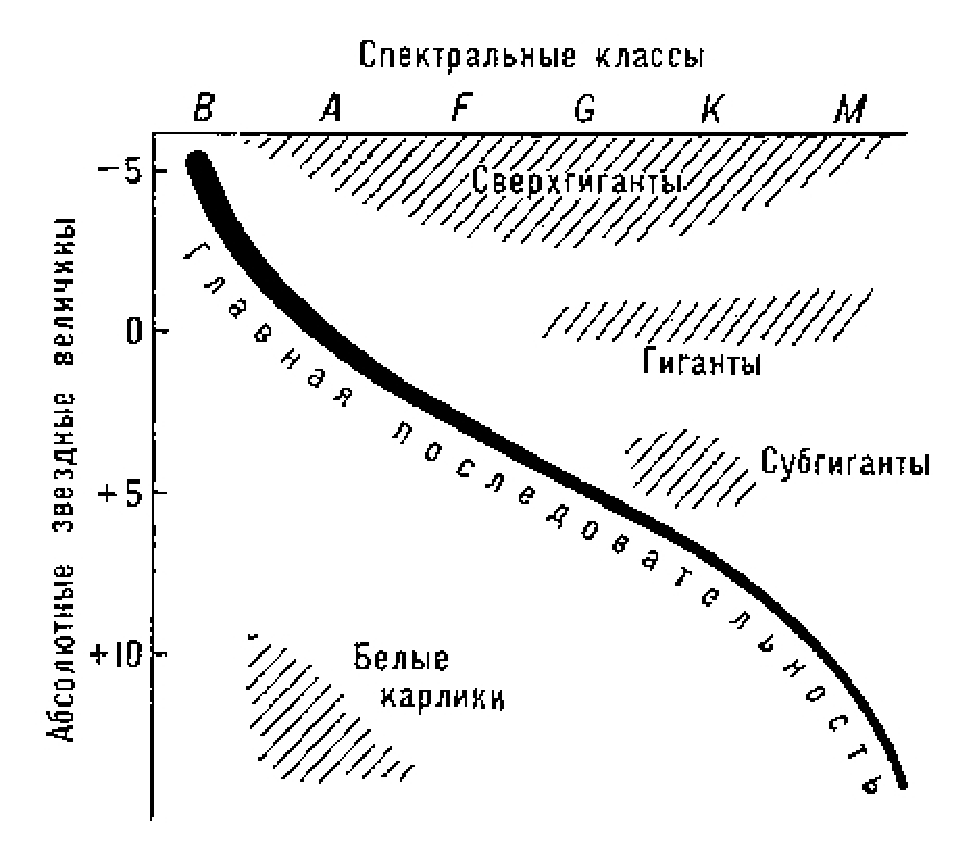
\includegraphics[width=4cm]{gr-example.eps}
            \end{center}
           
            \begin{itemize}
                \item Факторы: показатель цвета, абсолютная звездная величина
                \item Класс: класс светимости III, или V
                \item Алгоритм классификации: метод опорных векторов (Support Vector Machines, SVM)
            \end{itemize}
        \end{frame}        
        
        \begin{frame}{Классификатор}
            \begin{center}
                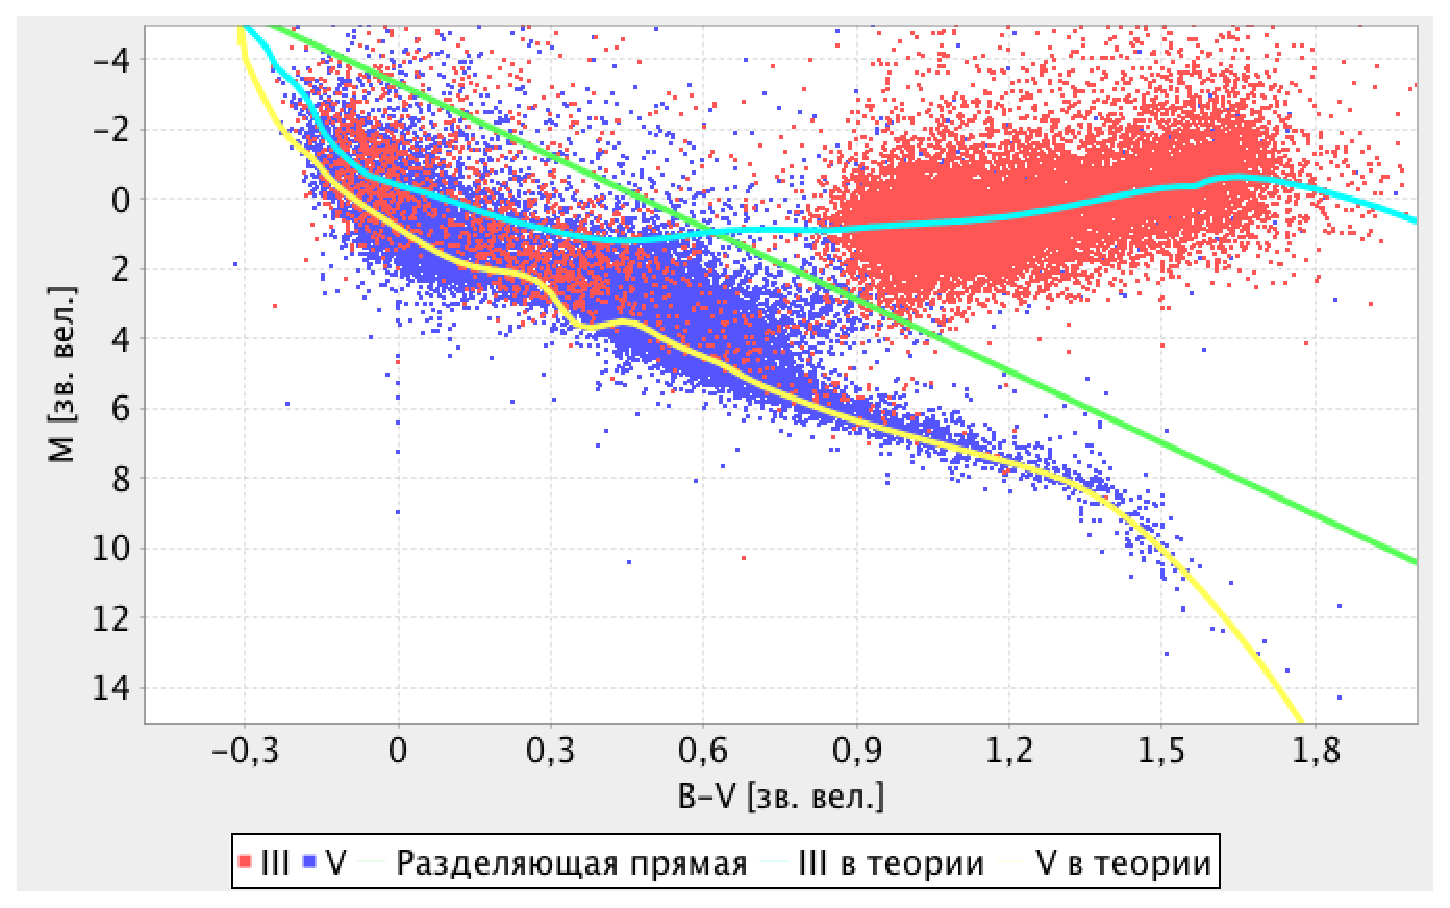
\includegraphics[width=11cm]{classify.eps}
            \end{center}             
        \end{frame}
        
        \begin{frame}{Качество классификации}
            Результаты кросс--валидации на 10 частях
            \begin{center}
            \begin{tabular} {| c | c | c | c |}
                \hline
                Решение классификатора $\rightarrow$   &    III   &    V    \\
                \hline
                III    &    16636    &    1992    \\
                \hline
                V       &    783    &    20396    \\
                \hline
            \end{tabular}
            
            ~\\~\\
            
            \begin{tabular} {| c | c | c | c |}
                \hline
                Класс    &    Точность   &    Полнота    &    F1-мера     \\
                \hline
                III      &    95\%   &   89\%    &    92\%     \\
                \hline
                V        &    91\%   &    96\%    &    93\%        \\
                \hline
            \end{tabular}
            \end{center}
        \end{frame}                  
        
        \begin{frame}{Результат}
            \begin{center}
                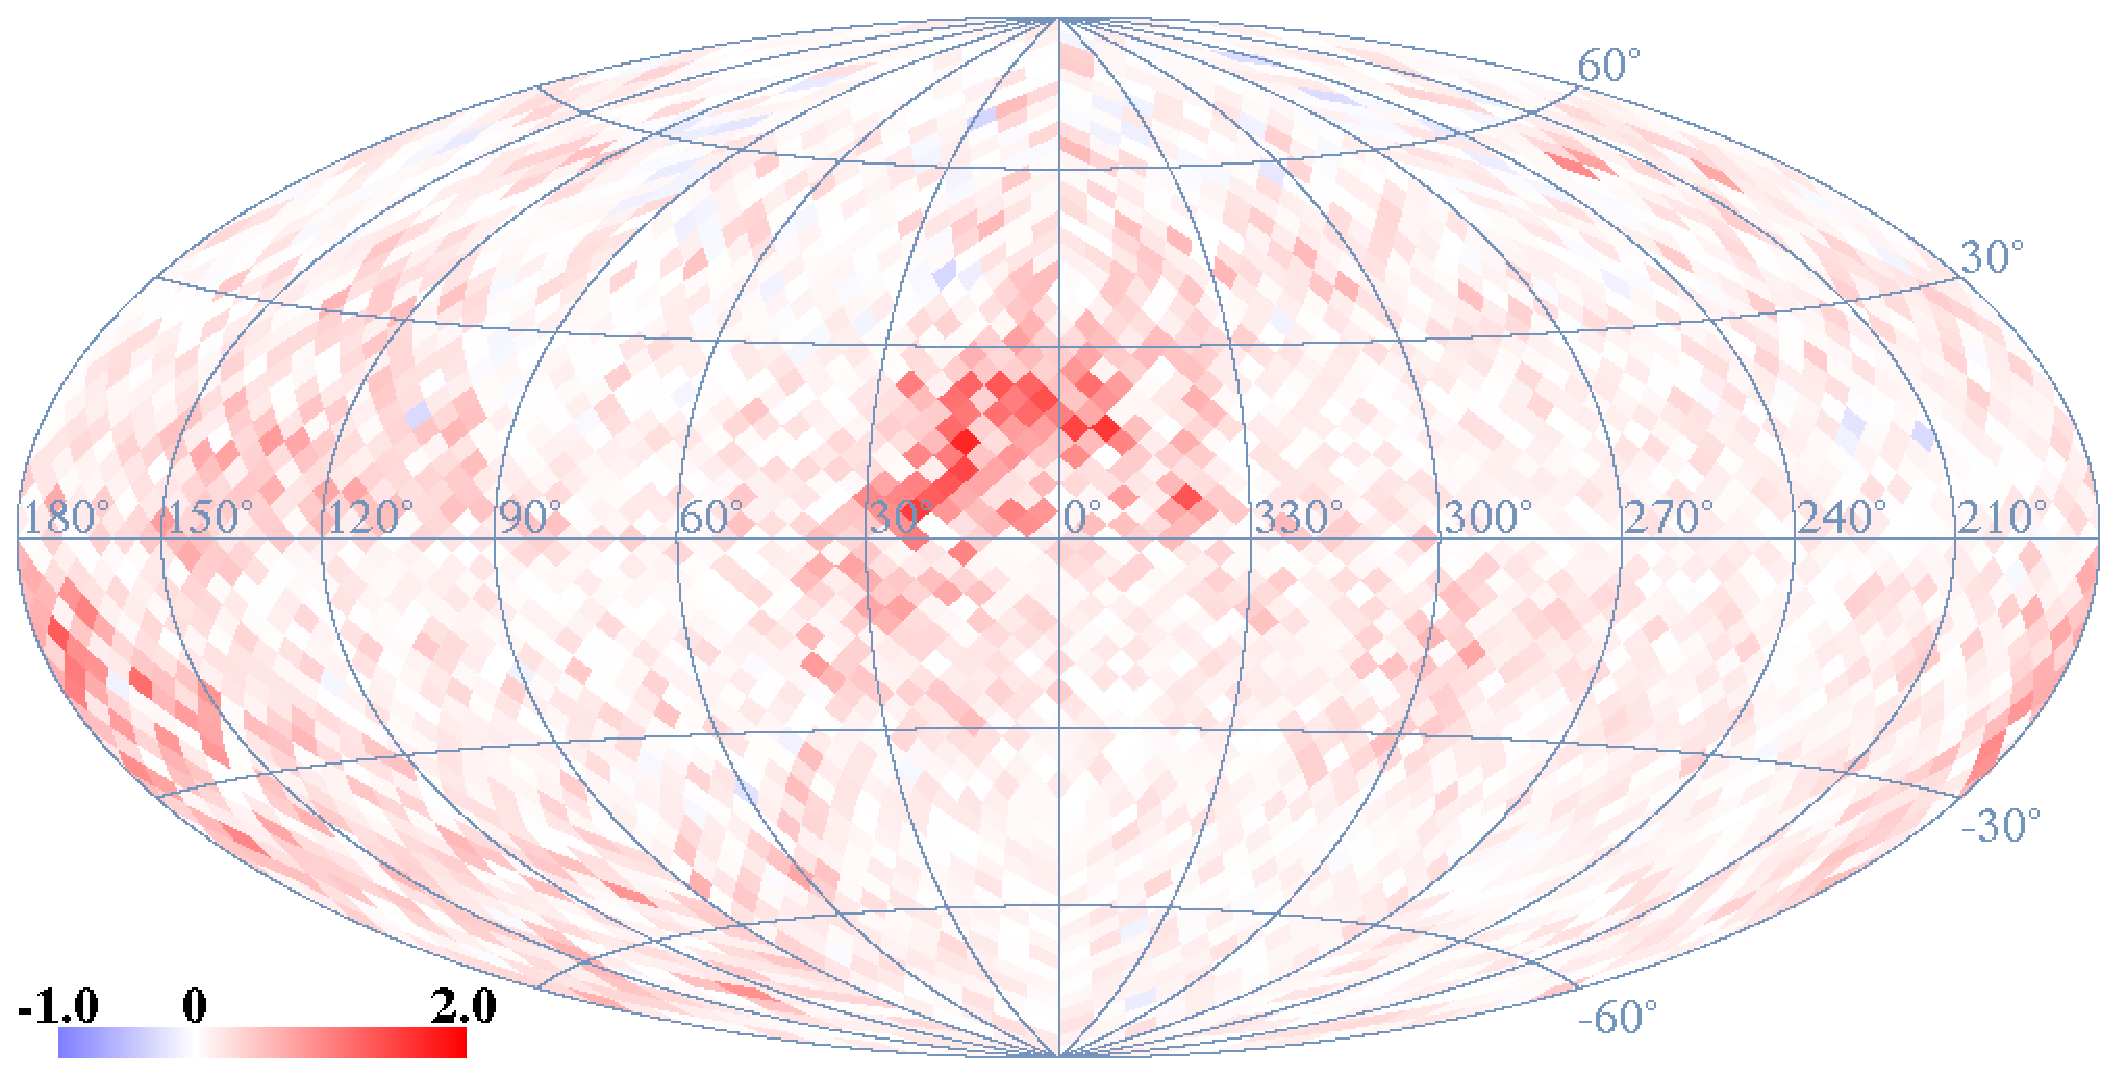
\includegraphics[width=11cm]{map-k.eps}
            \end{center}             
        \end{frame}
        
        \begin{frame}{Что дальше?}
            \begin{center}
                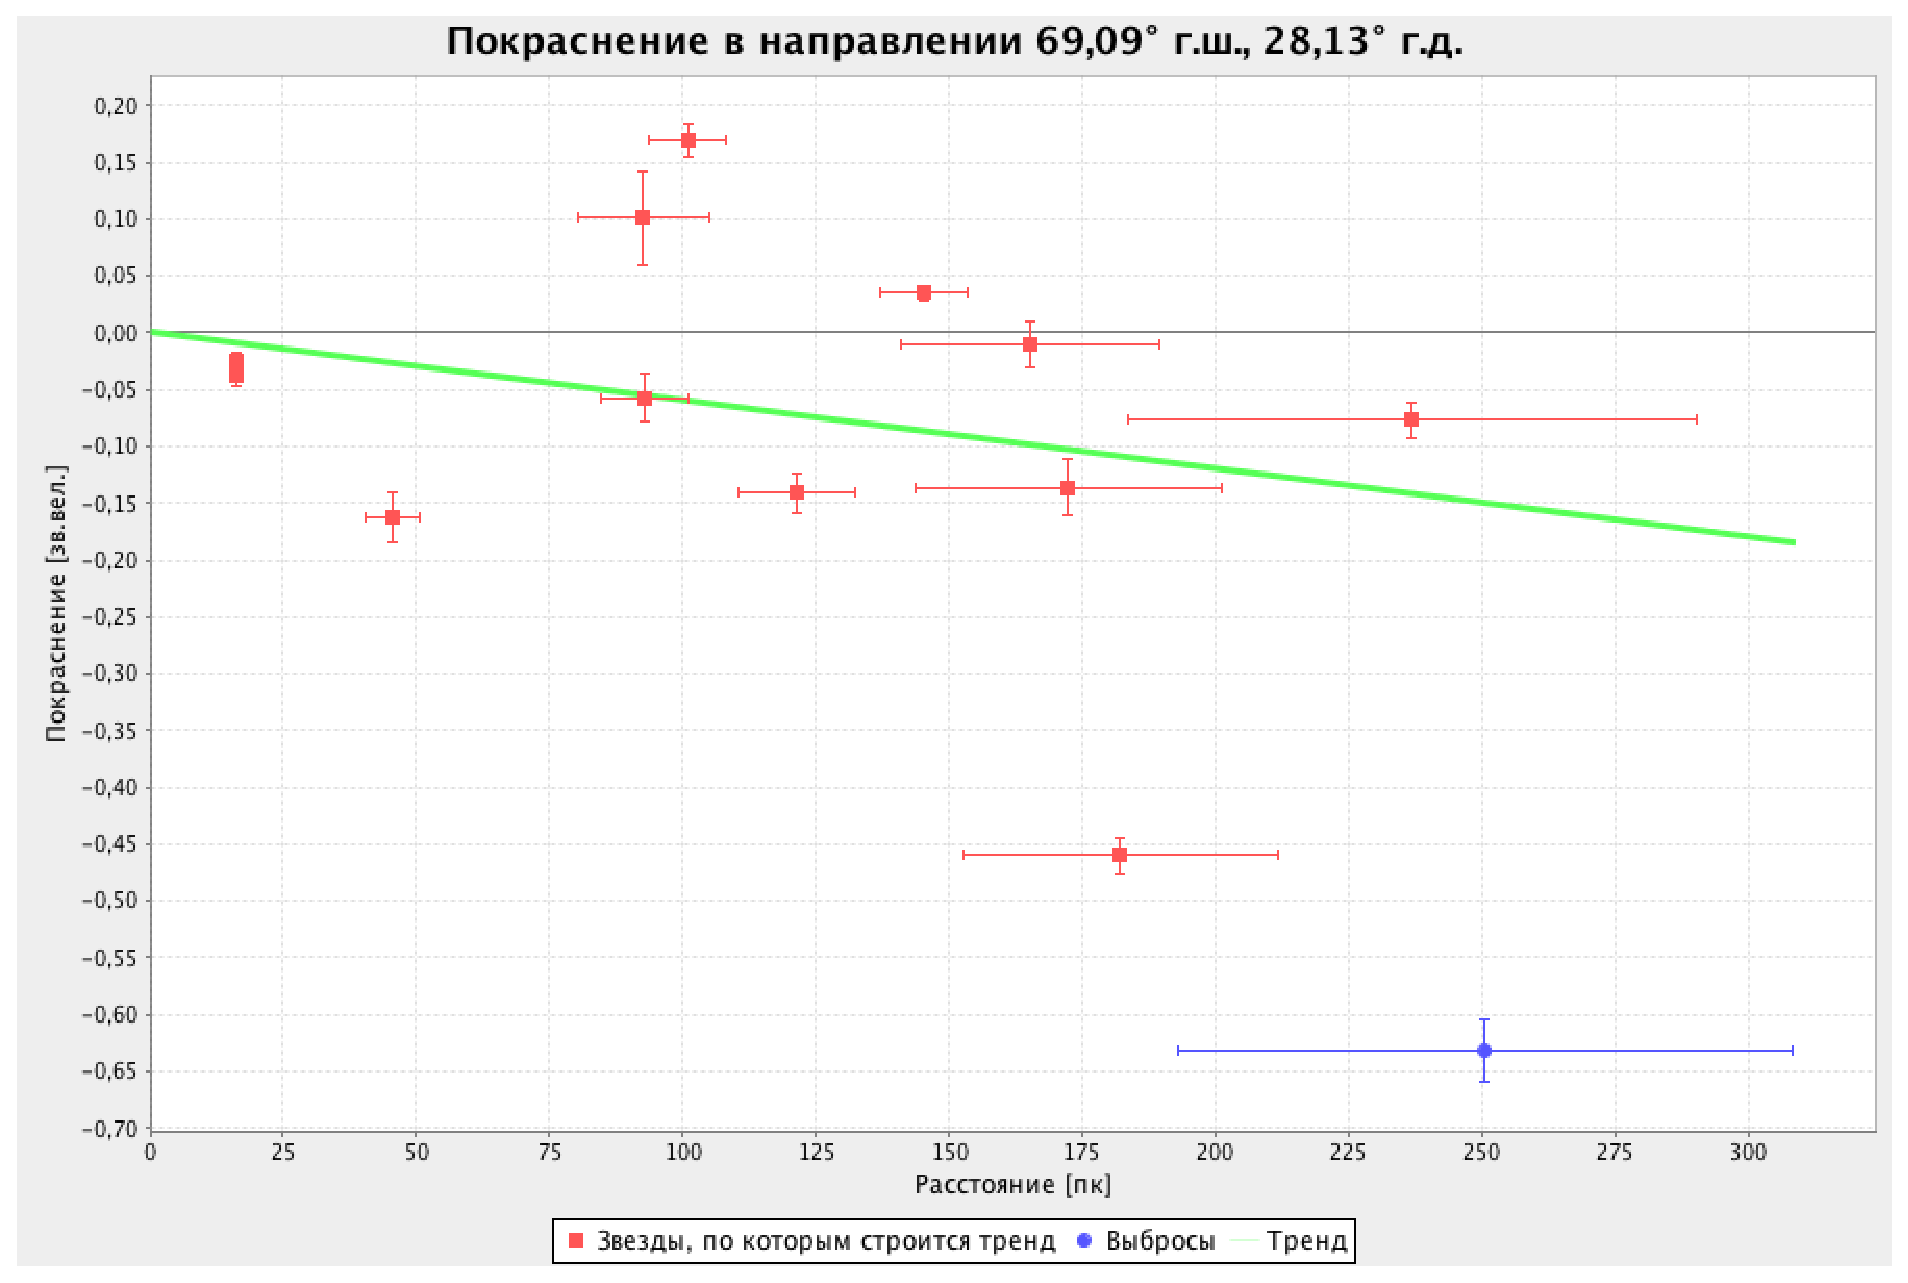
\includegraphics[width=10cm]{real-4-k.eps}
            \end{center}  
            $$E_{B - V} + 3 \sigma_{E_{B - V}} < 0$$
        \end{frame} 
        
	
        \begin{frame}{Q\&A}
            \begin{center}
                Спасибо за внимание!\\
                \href{https://github.com/amosov-f/dust-detection}{github.com/amosov-f/dust-detection}
            \end{center}
        \end{frame}

\end{document}